% !TEX root = ../main.tex
% 本文件由 build-tex.sh 从 09-DSP指南-第9章中译.md 生成，改内容请改 md 后重新生成

\chapter{DFT 的应用}\label{ch-09}

离散傅里叶变换（Discrete Fourier
Transform，DFT）是数字信号处理中最重要的工具之一。本章讨论它的三种常见用法。第一，DFT
可以计算信号的频谱(frequency
spectrum)。这是直接考察编码在各正弦分量的频率、相位和幅度中的信息。例如，人的语音和听觉用的就是这种编码方式的信号。第二，DFT
可以由系统的冲激响应求出系统的频率响应(frequency
response)，反过来也行。这让我们可以在频域里分析系统，就像卷积让我们可以在时域里分析系统一样。第三，DFT
可以作为更复杂的信号处理技术中的一个中间步骤。最经典的例子是 FFT
卷积(FFT convolution)，一种比常规方法快几百倍的卷积算法。

\section{信号的频谱分析}

信息编码在构成信号的正弦波里，这种情况非常普遍。自然产生的信号是这样，人造的信号也是这样。我们的宇宙里有许多东西在振荡。例如，语音来自人的声带振动；恒星和行星绕自身的轴自转、彼此绕转时，亮度会发生变化；船的螺旋桨让水产生周期性的位移，等等。对这些信号来说，时域波形的形状并不重要，关键信息在各正弦分量的频率、相位和幅度里。DFT
就是用来提取这些信息的。

举个例子来说明。假设我们想研究在海洋中传播的声音。首先，把一个麦克风放进水里，把得到的电信号放大到合适的电平，比如几伏。然后用一个模拟低通滤波器去掉
80 赫兹以上的所有频率，这样信号就能以每秒 160
个采样的速率数字化。采集并存储了几千个采样之后，下一步做什么？

第一件事就是看看数据。图 9-1a 是我们这个假想实验中的 256
个采样。能看到的只是一个满是噪声的波形，人眼从中看不出什么信息。出于稍后会解释的原因，下一步是把这个信号乘以一条叫汉明窗(Hamming
window)的平滑曲线，见 (b)。（第 16 章给出了汉明窗和其他窗的公式，见公式
16-1、16-2 和图 16-2a。）这样得到一个 256
点的信号，两端附近的采样幅度被压低了，见 (c)。

做 DFT 并转换成极坐标形式，得到 (d) 中 129
点的频谱。遗憾的是，它看起来也是一团乱糟糟的噪声。这是因为原来 256
个点里没有足够的信息，得不到一条规整的曲线。用更长的 DFT
对这个问题毫无帮助。例如，用 2048 点 DFT，频谱就有 1025 个采样。虽然原来
2048
个点包含更多信息，但频谱里采样数也按同样倍数增加，把信息摊薄了。更长的
DFT 提供更好的频率分辨率(frequency resolution)，但噪声水平不变。

办法是用更多的原始信号，同时不增加频谱的点数。具体做法是把输入信号切成许多段
256 点的片段。每段都乘以汉明窗，做 256 点
DFT，转换成极坐标形式。然后把得到的这些频谱取平均，形成一个 129
点的频谱。图 (e) 是对 100 个像 (d)
那样的频谱取平均的例子。改善是显而易见的：噪声降到了能看出信号有趣特征的水平。用这种方式取平均的只是频域的幅度；相位通常丢掉，因为它不含有用的信息。随机噪声按段数的平方根成比例减小。100
段比较典型，有些应用为了让微弱的特征显现出来，可能要对几百万段取平均。

还有第二种降低频谱噪声的方法。先做一个非常长的 DFT，比如 16,384
点。得到的频谱分辨率很高（8193
个采样），但噪声很大。再用一个低通数字滤波器把频谱平滑一下，以牺牲分辨率为代价降低噪声。例如，最简单的数字滤波器可以把原始频谱中
64
个相邻采样取平均，作为滤波后频谱的一个采样。算一算就知道，这和第一种方法给出的噪声与分辨率大致相同------相当于把
16,384 个点切成 64 段、每段 256 点。

该用哪种方法？第一种更容易，因为不需要数字滤波器。第二种有可能性能更好，因为可以对数字滤波器进行定制，优化噪声与分辨率之间的取舍。不过，这点性能提升很少值得费这个劲。因为噪声和分辨率都可以靠使用更多的输入数据来改善。例如，设想把采集到的数据切成
10,000 段，每段 16,384 个采样。这样得到的频谱分辨率高（8193
点），噪声也低（10,000
次平均）。问题解决了！因此，本章的讨论只看分段平均法。

\begin{figure}[htbp]
\centering
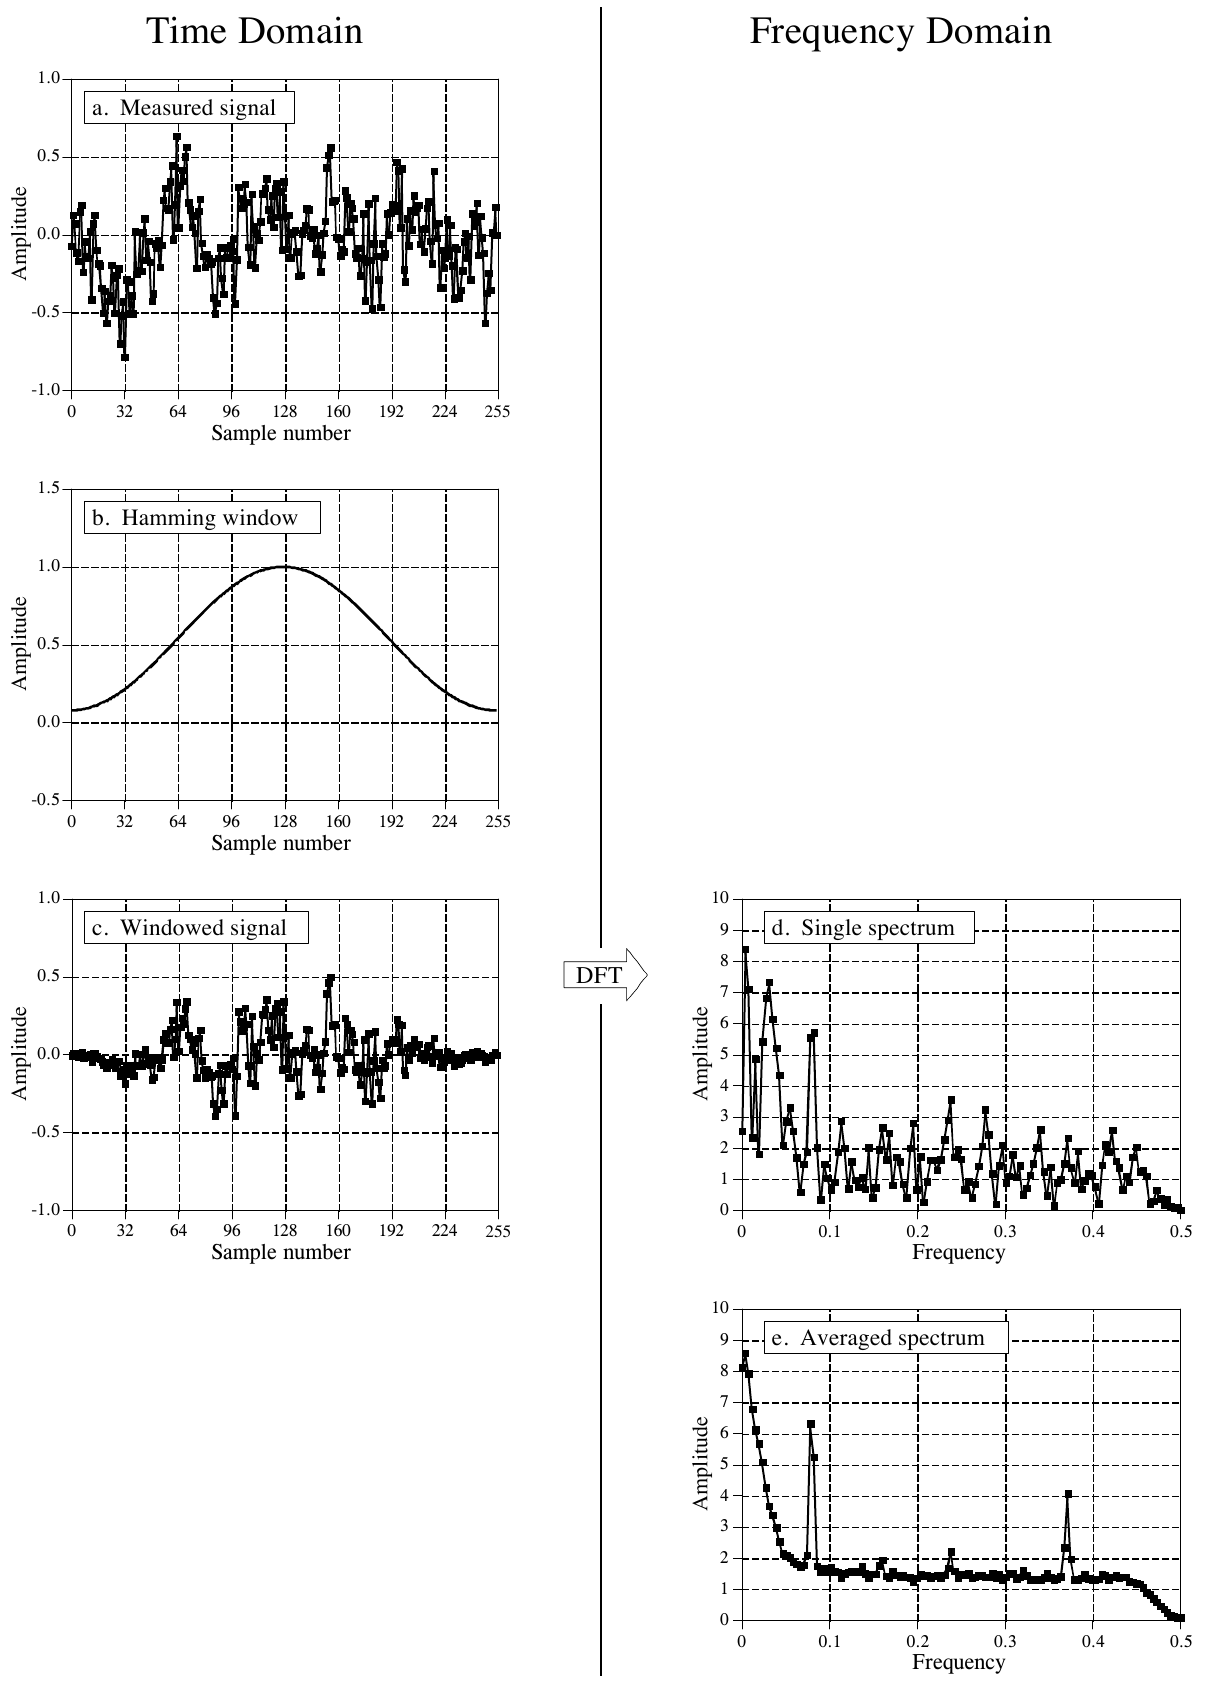
\includegraphics[width=1.000\linewidth,height=0.8\textheight,keepaspectratio]{assets/ch09/fig9-01.png}
\caption*{\textbf{图 9-1　频谱分析的一个例子。} (a) 是以每秒 160
个采样的速率从一个（模拟的）水下麦克风采得的 256 个采样。这个信号乘以
(b) 中的汉明窗，得到 (c) 中加窗后的信号。用 DFT
求出加窗信号的频谱，显示在 (d) 中（只画幅度）。对 100
个这样的频谱取平均可以降低随机噪声，得到 (e) 中的平均频谱。 （Time
Domain = 时域，Frequency Domain = 频域；a. Measured signal =
测得的信号；b. Hamming window = 汉明窗；c.~Windowed signal =
加窗后的信号；d.~Single spectrum = 单次频谱；e. Averaged spectrum =
平均频谱。Amplitude = 幅度，Sample number = 采样序号，Frequency =
频率。原书图注排在左下角空白处，裁图时已去掉，译文见上。）}
\end{figure}

图 9-2
是我们这个水下麦克风的一个频谱示例，展示了采集到的信号的频谱中常见的几种特征。先别管那些尖峰。在
10 到 70 赫兹之间，信号是一段比较平坦的区域。这叫白噪声(white
noise)，因为它包含等量的所有频率，就像白光一样。它源于时域波形上的噪声在采样之间互不相关(uncorrelated)。也就是说，知道某一个采样上的噪声值，对其他任何采样上的噪声值都提供不了任何信息。例如，电子电路中电子的随机运动就会产生白噪声。举个更熟悉的例子，淋浴时水花打在地上的声音就是白噪声。图
9-2 中的白噪声可能来自好几个源头，包括模拟电子电路，或者海洋本身。

70 赫兹以上，白噪声的幅度迅速下降。这是抗混叠滤波器(antialias
filter)滚降(roll-off)的结果。理想的滤波器会让 80
赫兹以下的所有频率通过，挡住以上的所有频率。实际上不可能做到完全陡峭的截止，你应该会看到这种逐渐的下降。如果没看到，就要怀疑出现了混叠问题。

大约 10 赫兹以下，噪声迅速上升，这是由一种叫 1/f 噪声（1/f noise，读作
one-over-f noise）的奇特现象造成的。1/f
噪声是个谜。人们在非常不同的系统里都测到过它，比如高速公路上的车流密度和晶体管里的电子噪声。只要看到足够低的频率，大概在所有系统里都能测到它。尽管它这么普遍，研究者至今没有得出关于
1/f
噪声的一般理论和认识。在某些具体系统里，这种噪声的成因是可以确定的；但这并没有回答为什么
1/f 噪声无处不在。对常见的模拟电子电路和大多数物理系统来说，白噪声和 1/f
噪声的分界大约在 1 到 100 赫兹之间。

\begin{figure}[htbp]
\centering
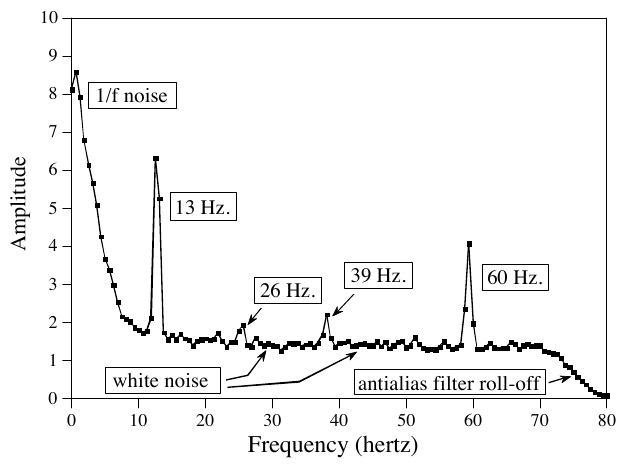
\includegraphics[width=0.517\linewidth,height=0.8\textheight,keepaspectratio]{assets/ch09/fig9-02.png}
\caption*{\textbf{图 9-2　频谱示例。} 采集到的信号的频谱中会出现三类特征：(1)
随机噪声，比如白噪声和 1/f 噪声；(2)
干扰信号，来自电源线、开关电源、广播电视台、微音效应等；(3)
真正的信号，通常表现为一个基频加上若干谐波。这个示例频谱（只画幅度）展示了其中几种特征。
（1/f noise = 1/f 噪声，white noise = 白噪声，antialias filter roll-off
= 抗混叠滤波器的滚降；13 Hz.、26 Hz.、39 Hz.、60 Hz.
为各峰的频率。Amplitude = 幅度，Frequency (hertz) =
频率（赫兹）。原书图注排在左侧，裁图时已去掉，译文见上。）}
\end{figure}

现在来看图 9-2 中的尖峰。最容易解释的是 60
赫兹那个，它是市电造成的电磁干扰。由于电源线的波形不是完美的正弦波，还应该会在这个频率的倍数（120、180、240
赫兹等）处看到较小的峰。在 25～40 kHz
之间也常能看到干扰峰，这是开关电源设计者偏爱的频段。附近的广播和电视台会在兆赫范围产生干扰峰。系统中的部件受到震动时也会振动，造成低频峰。这叫微音效应(microphonics)，通常在
10 到 100 赫兹产生峰。

现在来看真正的信号。在 13 赫兹有一个很强的峰，26 和 39
赫兹有较弱的峰。下一章会讲到，这是一个非正弦的周期波形的频谱。13
赫兹的峰叫基频(fundamental frequency)，26 和 39
赫兹的峰分别叫二次谐波和三次谐波(harmonic)。你还会预期在 13
赫兹的其他倍数处找到峰，比如 52、65、78 赫兹等。在图 9-2
中看不到它们，是因为它们被埋在白噪声里了。例如，这个 13
赫兹的信号可能是一艘潜艇的三叶螺旋桨以每秒 4.33
转旋转产生的。这正是被动声呐(passive
sonar)的原理：根据水下声音的频率和谐波成分来识别它们。

假设有几个峰靠得很近，如图 9-3
所示。有两个因素限制了能得到的频率分辨率，也就是峰能靠多近而不合并成一个。第一个因素是
DFT 的长度。N 点 DFT 产生的频谱由 N/2 + 1
个采样组成，均匀分布在零到采样频率的一半之间。要分开两个靠得很近的频率，采样间距必须小于两个峰之间的距离。例如，512
点 DFT 足以分开图 9-3 中的两个峰，而 128 点 DFT 不行。

\begin{figure}[htbp]
\centering
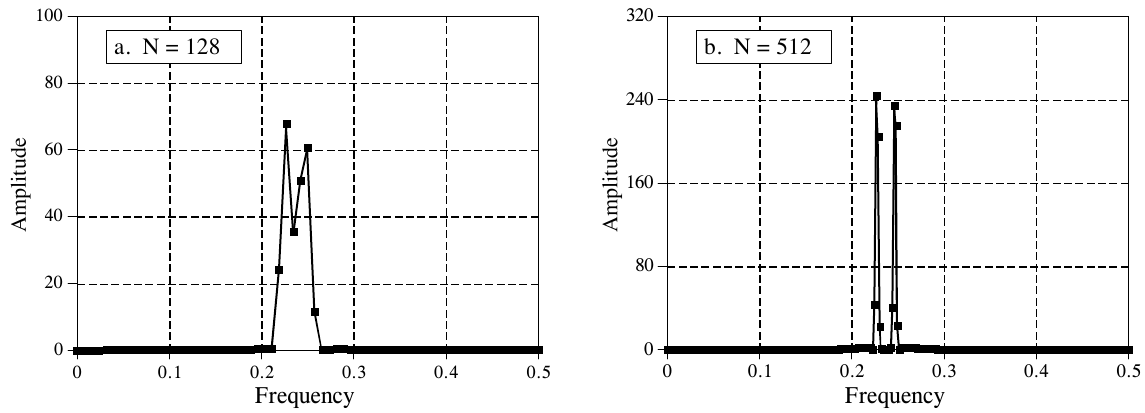
\includegraphics[width=0.954\linewidth,height=0.8\textheight,keepaspectratio]{assets/ch09/fig9-03.png}
\caption*{\textbf{图 9-3　频谱的分辨率。} DFT
越长，分开靠得很近的特征的能力越强。在这几个示例幅度谱中，128 点 DFT
分辨不出两个峰，而 512 点 DFT 可以。 （a. N = 128；b. N = 512。Amplitude
= 幅度，Frequency = 频率。）}
\end{figure}

限制分辨率的第二个因素更微妙。设想一个信号，由两个频率只差一点点的正弦波相加而成。在这个信号的一小段上，比如几个周期内，波形看起来就像一个单一的正弦波。两个频率越接近，这一段就必须越长，才能断定存在不止一个频率。换句话说，信号的长度限制了频率分辨率。这与第一个因素不同，因为输入信号的长度不必与
DFT 的长度相同。例如，一个 256 点的信号可以补零到 2048 点长。做 2048 点
DFT 得到 1025
个采样的频谱。补进去的零不改变频谱的形状，只是在频域里提供了更多的采样。尽管采样这么密，分开靠近的峰的能力只比用
256 点 DFT 好一点点。当 DFT
与输入信号等长时，分辨率受这两个因素的限制大约相当。我们稍后会再回到这个问题。

下一个问题：如果输入信号中含有一个频率位于两个基函数之间的正弦波，会怎样？图
9-4a
给出了答案。这是一个由两个正弦波组成的信号的频谱，其中一个的频率与某个基函数(basis
function)相同，另一个的频率在两个基函数之间。正如你所预期的，第一个正弦波表示为单独一个点。另一个峰比较难理解。由于它不能用单个采样表示，就变成了一个带有尾巴、尾巴延伸得很远的峰。

解决办法？像前面讲过的那样，在做 DFT 之前把信号乘以汉明窗。图 (b)
表明，加窗以后频谱在三个方面发生了变化。第一，两个峰变得更相像了。这是好事。第二，尾巴大大减小了。这也是好事。第三，窗让峰变宽，降低了频谱的分辨率。这是坏事。用
DSP 的行话说，窗在分辨率（峰的宽度）与频谱泄漏(spectral
leakage)（尾巴的幅度）之间提供了一种取舍。

\begin{figure}[htbp]
\centering
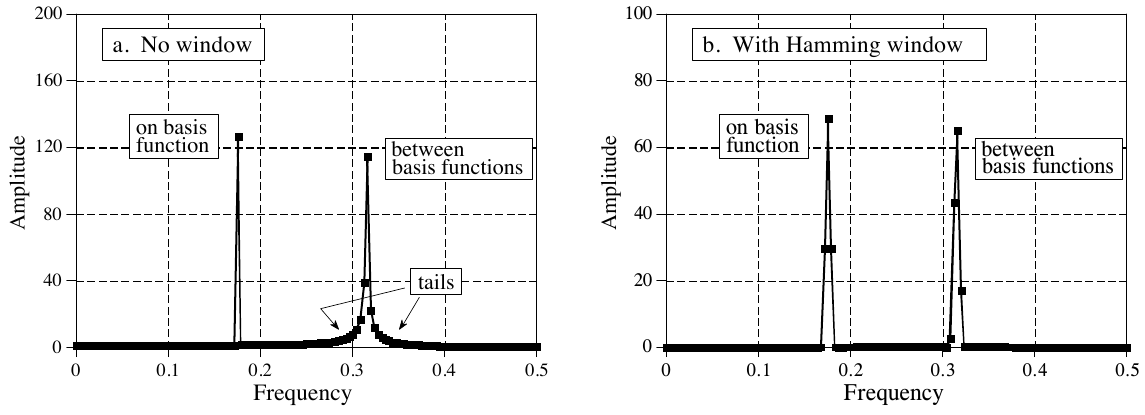
\includegraphics[width=0.954\linewidth,height=0.8\textheight,keepaspectratio]{assets/ch09/fig9-04.png}
\caption*{\textbf{图 9-4　在频谱分析中使用窗的例子。} (a)
是一个由两个正弦波组成的信号的频谱（只画幅度）。一个正弦波的频率恰好等于某个基函数，因此可以用单个采样表示；另一个的频率在两个基函数之间，导致峰带有尾巴。(b)
是同一个信号在做 DFT
之前加窗后的频谱。窗使两个峰看起来一样并减小了尾巴，但使峰变宽了。 （a.
No window = 不加窗；b. With Hamming window = 加汉明窗；on basis function
= 落在基函数上，between basis functions = 位于两个基函数之间，tails =
尾巴。Amplitude = 幅度，Frequency = 频率。）}
\end{figure}

\begin{quote}
\textbf{译注：} 原书图 9-4 的图注写的是 ``with a Blackman window
applied''（加布莱克曼窗），但正文和子图 (b) 的标签都是汉明窗(Hamming
window)。这里按正文和子图译作汉明窗。
\end{quote}

为了更详细地探讨其中的理论，设想一个无限长的离散正弦波，频率为采样率的
0.1。这个信号的频谱是一个无限窄的峰，其他所有频率都为零。当然，这个信号和它的频谱都无法放进数字计算机，因为一个无限长、一个无限窄。为了绕过这一点，我们从两个方面改变这个信号，这两方面都会使真实频谱失真。

第一，用一个窗去乘信号，从而截断信号中的信息。例如，一个 256
点的矩形窗(rectangular window)让 256
个点保留原值，而这个无限长信号中的其他所有采样都被设为零。同样，汉明窗除了把窗外的点都设为零以外，还会对保留下来的采样进行整形。这个信号仍然是无限长的，但只有有限个采样的值不为零。

这种加窗对频域有什么影响？第 10
章会讲到，两个时域信号相乘时，对应的频域是相卷积的。由于原来的频谱是一个无限窄的峰（即冲激函数），加窗信号的频谱就是窗的频谱平移到这个峰所在的位置。图
9-5
展示了用四种不同的窗时频谱峰会是什么样子。（如果需要复习分贝(dB)，可以先看第
14 章。）图 9-5a 是矩形窗的结果。(b) 和 (c)
是两种常用的窗------汉明窗和布莱克曼窗(Blackman
window)------的结果（前面说过，这两种窗的资料见公式 16-1、16-2 和图
16-2a）。

如图 9-5 所示，这些窗都使原频谱变差了：峰变宽，并添上了由许多旁瓣(side
lobe)组成的尾巴。这是只使用原时域信号一部分的必然结果。从这里可以看出三种窗之间的取舍。布莱克曼窗的主瓣(main
lobe)最宽（坏），但尾巴的幅度最低（好）。矩形窗的主瓣最窄（好），但尾巴最大（坏）。汉明窗介于两者之间。

注意，图 9-5
中的频谱是连续曲线，而不是离散采样。加窗以后，时域信号仍然是无限长的，尽管其中大多数采样都是零。这意味着频谱在
0 到 0.5 之间由 \dspsym{∞}/2 + 1 个采样组成，也就和一条连续的线一样。

\begin{figure}[htbp]
\centering
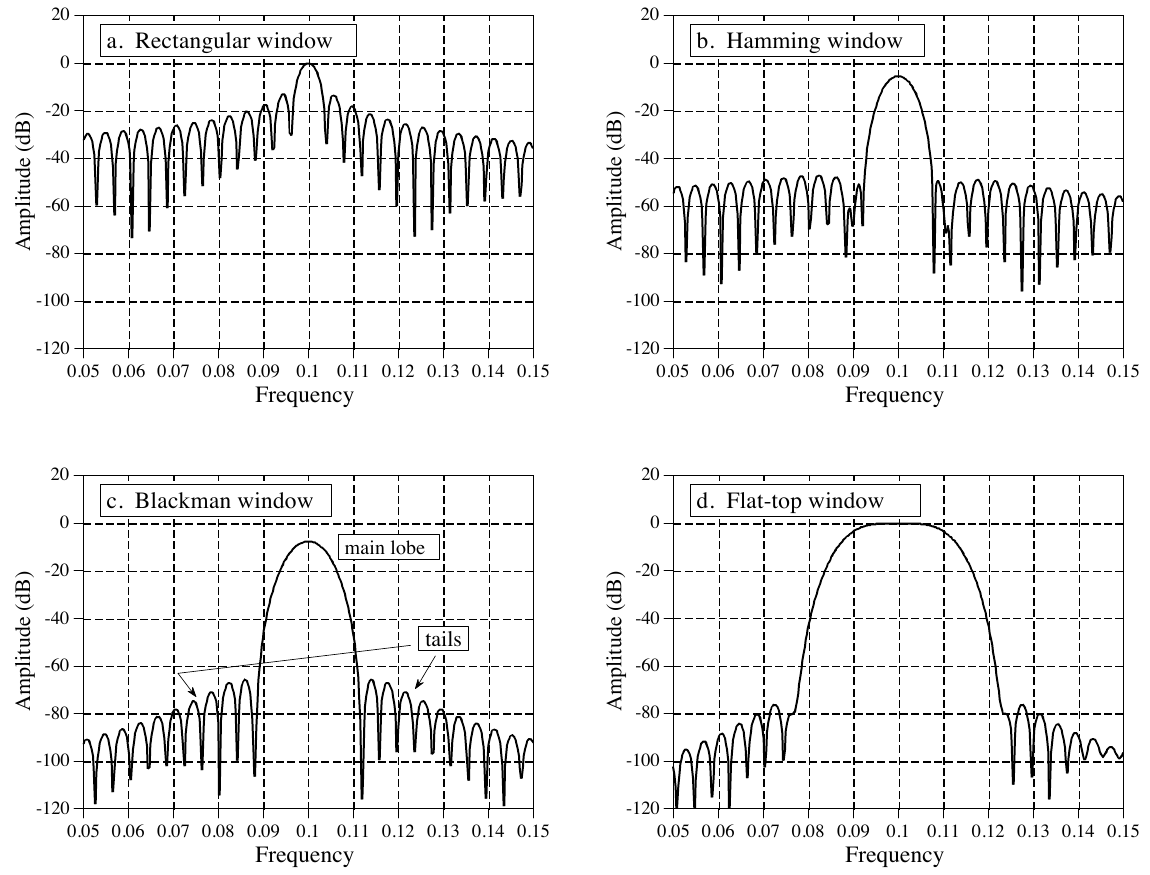
\includegraphics[width=0.958\linewidth,height=0.8\textheight,keepaspectratio]{assets/ch09/fig9-05.png}
\caption*{\textbf{图 9-5　用不同的窗时频谱峰的细节。}
频谱中的每个峰都是一个中央主瓣，四周是由旁瓣构成的尾巴。改变窗的形状，可以以主瓣变宽为代价降低旁瓣的幅度。矩形窗
(a) 的主瓣最窄，但旁瓣幅度最大。汉明窗 (b) 和布莱克曼窗 (c)
的旁瓣幅度较低，代价是主瓣较宽。平顶窗 (d)
用于必须精确测量峰的幅度的场合。这些曲线对应 255
点的窗；窗越长，峰按比例越窄。 （a. Rectangular window = 矩形窗；b.
Hamming window = 汉明窗；c.~Blackman window = 布莱克曼窗；d.~Flat-top
window = 平顶窗；main lobe = 主瓣，tails = 尾巴。Amplitude (dB) =
幅度（分贝），Frequency = 频率。）}
\end{figure}

这就引出了为了能在计算机中表示，需要对时域信号做的第二种修改：从信号中选取
N 个点。这 N
个点必须包含窗所确定的全部非零点，但也可以包含任意多个零。这样做的效果是对频谱的连续曲线进行采样。例如，如果
N 取 1024，频谱的连续曲线就在 0 到 0.5 之间被采样 513 次。如果 N
取得比窗长大得多，频域中的采样就会足够密，连续曲线的峰和谷都能在新频谱中保留下来。如果
N
取得和窗长一样，频谱中的采样较少，峰谷规则交替的图样就会变成不规则的尾巴，具体是什么样子取决于采样恰好落在哪里。这就解释了为什么图
9-4a 中的两个峰看起来不一样。图 9-4a 中的每个峰，都是对图 9-5a
中那条底层曲线的一次采样。尾巴有没有，取决于采样位置与峰、谷的相对关系。如果正弦波恰好与某个基函数相符，采样就恰好落在谷底，尾巴消失。如果正弦波位于两个基函数之间，采样就落在峰谷之间的某些位置，形成各种样子的尾巴。

这就引出了图 9-5d 所示的平顶窗(flat-top
window)。在某些应用中，频谱峰的幅度必须测得非常准。由于 DFT
的频谱是由采样构成的，没有什么能保证某个采样恰好落在峰顶。更可能的情况是，最近的那个采样稍稍偏离中心，得到的值比真实幅度低。解决办法是使用一种能让频谱峰顶部平坦的窗，确保总有一个或多个采样取到正确的峰值。如图
9-5d 所示，代价是主瓣非常宽，导致频率分辨率很差。

事实上，我们想要的平顶窗的形状，恰好和低通滤波器的滤波器核形状完全相同。后面的章节会讨论其中的理论原因；这里先给出这种技术的使用''菜谱''。第
16 章讨论一种叫加窗 sinc(windowed-sinc) 的低通滤波器。公式 16-4
描述了怎样生成它的滤波器核（我们要把它用作窗），图 16-4a
画出了这条曲线的典型形状。要用这个公式，需要知道两个参数的值：M 和
\(f_c\)。它们由下面的关系求出：\(M = N - 2\)，\(f_c = s/N\)，其中 N
是所用 DFT 的长度，s 是你希望峰的平坦部分上有几个采样（通常在 3 到 5
之间）。表 16-1
给出了计算这个滤波器核（也就是我们的窗）的程序，其中包含两个细微之处：归一化常数
K，以及怎样避免中心采样处除以零的错误。使用这种方法时要记住：时域中值为一的直流，会在频域中产生幅度为一的峰；但时域中幅度为一的正弦波，只会产生幅度为二分之一的频谱峰。（这在上一章的''合成：计算逆
DFT''一节讨论过。）

\section{系统的频率响应}

在时域中，用卷积来分析系统。在频域中也可以做类似的分析。利用傅里叶变换，每个输入信号都可以表示为一组余弦波，每个余弦波有确定的幅度和相移。同样，DFT
也可以把每个输出信号表示成类似的形式。这意味着任何线性系统都可以完全由它怎样改变通过它的余弦波的幅度和相位来描述。这些信息叫做系统的频率响应。由于冲激响应和频率响应都包含了关于系统的完整信息，两者之间必然一一对应。知道其中一个，就能算出另一个。冲激响应与频率响应之间的关系，是信号处理的基石之一：\textbf{系统的频率响应是其冲激响应的傅里叶变换。}图
9-6 展示了这些关系。

按照 DSP 的标准记法，冲激响应用小写变量，对应的频率响应用大写。由于 h{[}
{]} 是冲激响应的常用符号，频率响应就用 H{[}
{]}。系统在时域中用卷积描述，即
\(x[n] * h[n] = y[n]\)。在频域中，输入频谱乘以频率响应，得到输出频谱。写成公式：\(X[f] \times H[f] = Y[f]\)。也就是说，时域中的卷积对应频域中的乘法。

\begin{figure}[htbp]
\centering
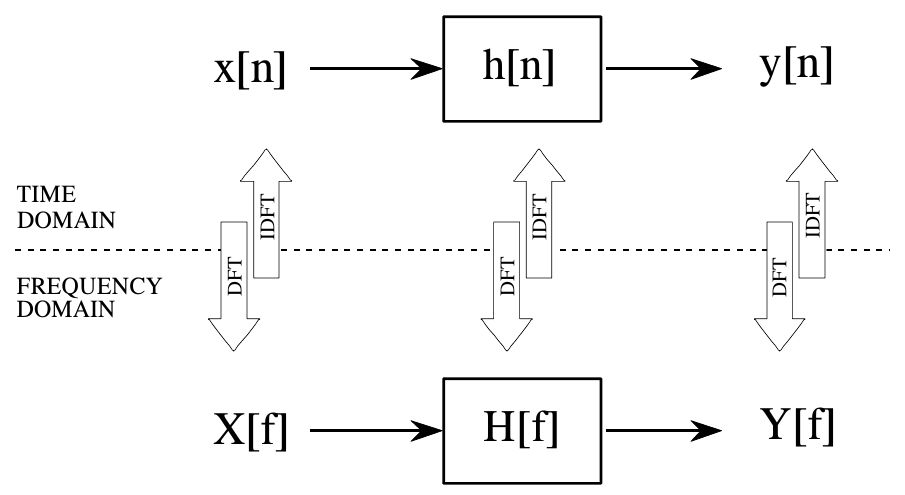
\includegraphics[width=0.754\linewidth,height=0.8\textheight,keepaspectratio]{assets/ch09/fig9-06.png}
\caption*{\textbf{图 9-6　比较系统在时域和频域中的运作。}
在时域中，输入信号与冲激响应卷积，得到输出信号，即
\(x[n] * h[n] = y[n]\)。在频域中，输入频谱乘以频率响应，得到输出频谱，即
\(X[f] \times H[f] = Y[f]\)。DFT 和逆 DFT 把两个域中的信号联系起来。
（TIME DOMAIN = 时域，FREQUENCY DOMAIN = 频域；DFT =
离散傅里叶变换，IDFT = 逆 DFT。）}
\end{figure}

图 9-7 是用 DFT 把系统的冲激响应转换成频率响应的一个例子。(a)
是系统的冲激响应。看这条曲线，你一点也看不出这个系统是做什么的。对这个冲激响应做
64 点 DFT，得到系统的频率响应，见
(b)。现在这个系统的作用就一目了然了：它让 0.2 到 0.3
之间的频率通过，挡住其他所有频率。这是一个带通滤波器(band-pass
filter)。也可以考察频率响应的相位，不过它更难解释，也没那么有意思。后面的章节会讨论它。

\begin{enumerate}
\def\labelenumi{(\alph{enumi})}
\setcounter{enumi}{1}
\tightlist
\item
  非常参差不齐，这是因为确定这条曲线的采样太少。在做 DFT
  之前给冲激响应补零，可以改善这种情况。例如，补零使冲激响应长 512
  个采样，如 (c) 所示，就得到 (d) 中分辨率更高的频率响应。
\end{enumerate}

\begin{figure}[htbp]
\centering
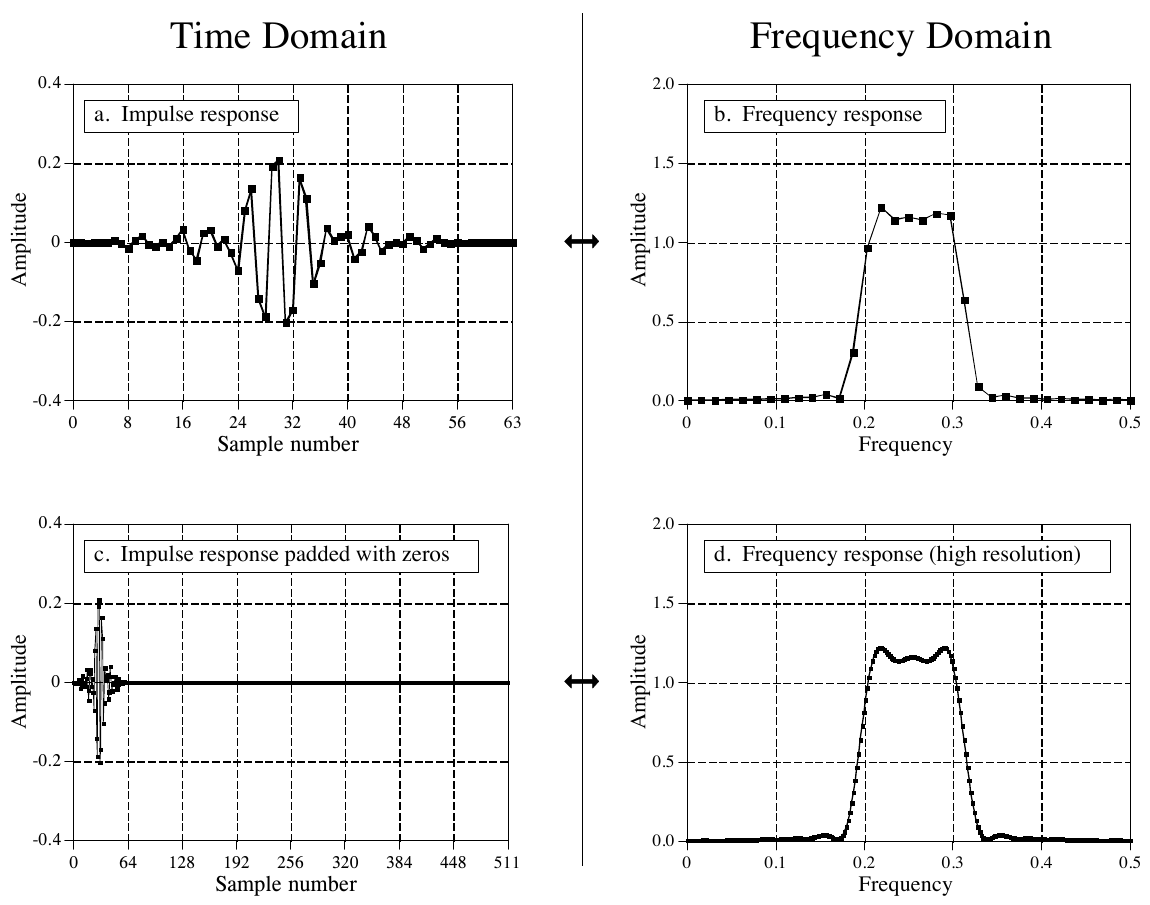
\includegraphics[width=0.958\linewidth,height=0.8\textheight,keepaspectratio]{assets/ch09/fig9-07.png}
\caption*{\textbf{图 9-7　由冲激响应求频率响应。} 利用 DFT，系统的冲激响应 (a)
可以变换成系统的频率响应 (b)。给冲激响应补零
(c)，可以在频率响应中得到更高的分辨率
(d)。本例只画了频率响应的幅度，相位的讨论推迟到下一章。 （Time Domain =
时域，Frequency Domain = 频域；a. Impulse response = 冲激响应；b.
Frequency response = 频率响应；c.~Impulse response padded with zeros =
补零后的冲激响应；d.~Frequency response (high resolution) =
频率响应（高分辨率）。Amplitude = 幅度，Sample number =
采样序号，Frequency = 频率。）}
\end{figure}

频率响应能得到多高的分辨率？答案是：无限高，只要你愿意给冲激响应补无限多个零。换句话说，除了
DFT
的长度，没有什么限制频率分辨率。这引出一个非常重要的概念：尽管冲激响应是离散信号，对应的频率响应却是连续的。对冲激响应做
N 点 DFT，得到这条连续曲线的 N/2 + 1 个采样。DFT
做得越长，分辨率越高，你对这条连续曲线长什么样的了解就越清楚。记住频率响应代表什么：余弦波通过系统时经历的幅度和相位变化。由于输入信号可以包含
0 到 0.5 之间的任何频率，系统的频率响应在这个范围内必须是一条连续曲线。

引入傅里叶变换家族的另一个成员------离散时间傅里叶变换（Discrete Time
Fourier Transform，DTFT），可以更好地理解这一点。考虑一个 N
个采样的信号通过 N 点 DFT，产生 N/2 + 1 个采样的频域。回忆上一章：DFT
把时域信号看作无限长、周期性的。也就是说，这 N
个点从负无穷到正无穷一遍又一遍地重复。现在考虑我们开始给时域信号补越来越多的零，以便在频域中得到越来越细的采样，会发生什么。补零使时域的周期变长，同时使频域的采样靠得更近。

现在把这推到极端：给时域信号补无限多个零。这在两个方面造成了不同的局面。第一，时域信号现在的周期无限长。换句话说，它变成了非周期信号。第二，频域的采样间距变得无限小。也就是说，它变成了连续信号。这就是
DTFT：把时域中离散的非周期信号，变成频域中一条连续曲线的过程。用数学的话说，系统的频率响应是对它的冲激响应做
DTFT 得到的。由于这在计算机里做不到，就用 DFT
来计算真实频率响应的一组采样。这就是你在计算机里做的（DFT）与你用数学公式做的（DTFT）之间的区别。

\section{通过频域做卷积}

假设你讨厌卷积。给你一个输入信号和一个冲激响应，要求出输出信号，你会怎么办？图
9-8
给出了一个答案：把两个信号变换到频域，相乘，再把结果变换回时域。这就把一次卷积换成了两次
DFT、一次乘法和一次逆
DFT。尽管中间步骤截然不同，输出和标准卷积算法完全相同。

有人讨厌卷积到愿意费这个周折吗？答案是有。避开卷积有两个原因。第一，卷积在数学上很难处理。例如，假设给你一个系统的冲激响应和它的输出信号，怎样算出输入信号是什么？这叫解卷积(deconvolution)，在时域里几乎无法理解。然而在频域里，解卷积可以用一次简单的除法------乘法的逆运算------来完成。只要傅里叶变换的复杂度低于卷积的复杂度，频域就有吸引力。这不是你更喜欢哪个的问题，而是你更不讨厌哪个的问题。

避开卷积的第二个原因是计算速度。例如，假设你设计了一个数字滤波器，它的核（冲激响应）有
512 个采样。在一台 200
MHz、使用浮点数的个人计算机上，用标准卷积算法，输出信号的每个采样大约需要一毫秒来计算。换句话说，系统的吞吐量只有每秒约
1000 个采样。这对高保真音频来说慢了 40 倍，对电视画质的视频来说慢了
10,000 倍！

标准卷积算法慢，是因为必须计算大量的乘法和加法。遗憾的是，仅仅用 DFT
把问题搬到频域里毫无帮助。计算 DFT
所需的运算量，和直接计算卷积一样多。1960 年代初快速傅里叶变换（Fast
Fourier Transform，FFT）的提出，使这个问题取得了突破。FFT 是一种快速计算
DFT 的巧妙算法。利用
FFT，通过频域相乘做卷积，可以比常规卷积快几百倍。要算好几个小时的问题，缩短到只要几分钟。这就是为什么人们对
FFT 和在频域中处理信号如此兴奋。FFT 将在第 12 章介绍，FFT 卷积的方法在第
18 章介绍。眼下先集中精力理解信号怎样通过频域相乘来卷积。

\begin{figure}[htbp]
\centering
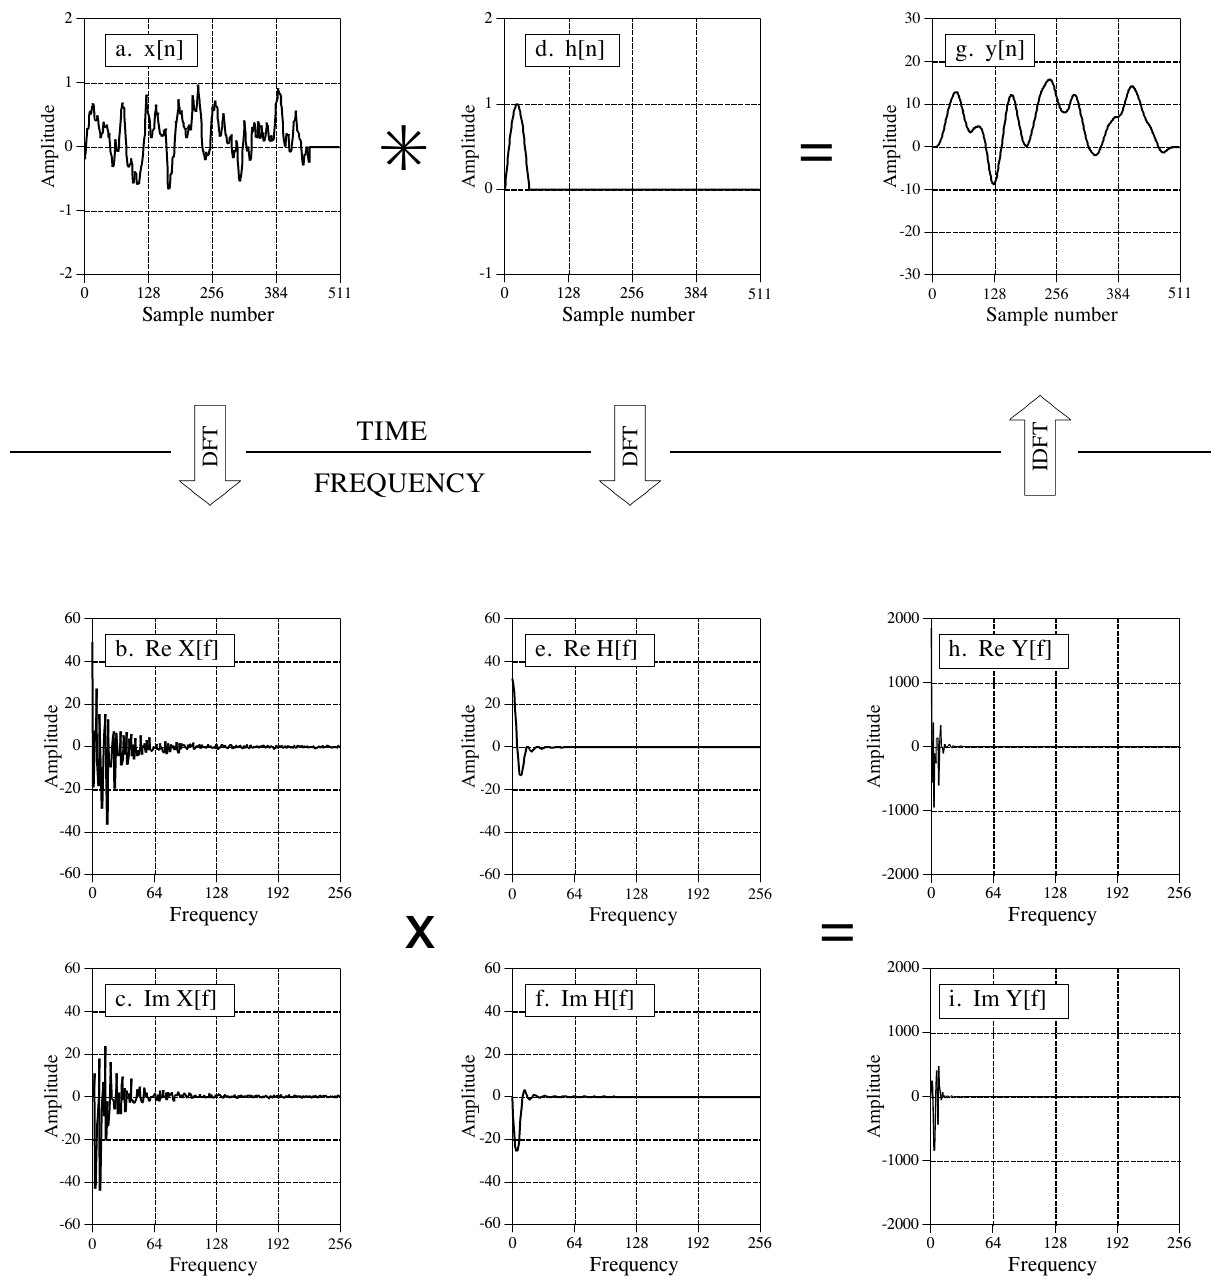
\includegraphics[width=1.000\linewidth,height=0.8\textheight,keepaspectratio]{assets/ch09/fig9-08.png}
\caption*{\textbf{图 9-8　频域卷积。} 在时域中，x{[}n{]} 与 h{[}n{]} 卷积得到
y{[}n{]}，如 (a)、(d)、(g) 所示。同样的过程也可以在频域中完成：用 DFT
求出输入信号的频谱 (b)、(c) 和系统的频率响应
(e)、(f)，把这两个频域信号相乘，得到输出信号的频谱 (h)、(i)，再用逆 DFT
求出输出信号 (g)。 （a. x{[}n{]}；d.~h{[}n{]}；g. y{[}n{]}；b. Re
X{[}f{]}；c.~Im X{[}f{]}；e. Re H{[}f{]}；f.~Im H{[}f{]}；h. Re
Y{[}f{]}；i. Im Y{[}f{]}。TIME = 时域，FREQUENCY = 频域；\dspsym{∗}
为卷积，x 为相乘。Amplitude = 幅度，Sample number = 采样序号，Frequency
= 频率。）}
\end{figure}

首先，需要定义一个频域信号怎样乘以另一个频域信号，即
\(X[f] \times H[f] = Y[f]\)
是什么意思。在极坐标形式下，幅度相乘：\(\mathrm{Mag}\,Y[f] = \mathrm{Mag}\,X[f] \times \mathrm{Mag}\,H[f]\)；相位相加：\(\mathrm{Phase}\,Y[f] = \mathrm{Phase}\,X[f] + \mathrm{Phase}\,H[f]\)。要理解这一点，可以设想一个具有某个幅度和相位的余弦波进入系统。同样，输出信号也是一个具有某个幅度和相位的余弦波。频率响应的极坐标形式，直接描述了这两个幅度之间以及两个相位之间的关系。

用直角坐标形式做频域乘法时，实部和虚部之间会有交叉项。例如，进入系统的正弦波在输出中可以同时产生余弦波和正弦波。用直角坐标记法做频域信号相乘：

\textbf{公式
9-1}　频域信号在直角坐标形式下的乘法：\(Y[f] = X[f] \times H[f]\)。

\[\mathrm{Re}\,Y[f] = \mathrm{Re}\,X[f]\,\mathrm{Re}\,H[f] - \mathrm{Im}\,X[f]\,\mathrm{Im}\,H[f]\]

\[\mathrm{Im}\,Y[f] = \mathrm{Im}\,X[f]\,\mathrm{Re}\,H[f] + \mathrm{Re}\,X[f]\,\mathrm{Im}\,H[f]\]

重点放在用极坐标记法理解乘法、理解余弦波通过系统的思路上。然后只需接受：同样的运算在直角坐标形式下进行，就会得到这些更复杂的式子。再比如，看看一个频域信号除以另一个频域信号。在极坐标形式下，频域信号的除法用乘法所用运算的逆运算来实现。要计算
\(H[f] = Y[f] / X[f]\)，就把幅度相除、相位相减，即
\(\mathrm{Mag}\,H[f] = \mathrm{Mag}\,Y[f] / \mathrm{Mag}\,X[f]\)，\(\mathrm{Phase}\,H[f] = \mathrm{Phase}\,Y[f] - \mathrm{Phase}\,X[f]\)。在直角坐标形式下则变成：

\textbf{公式 9-2}　频域信号在直角坐标形式下的除法，其中
\(H[f] = Y[f] / X[f]\)。

\[\mathrm{Re}\,H[f] = \frac{\mathrm{Re}\,Y[f]\,\mathrm{Re}\,X[f] + \mathrm{Im}\,Y[f]\,\mathrm{Im}\,X[f]}{\mathrm{Re}\,X[f]^2 + \mathrm{Im}\,X[f]^2}\]

\[\mathrm{Im}\,H[f] = \frac{\mathrm{Im}\,Y[f]\,\mathrm{Re}\,X[f] - \mathrm{Re}\,Y[f]\,\mathrm{Im}\,X[f]}{\mathrm{Re}\,X[f]^2 + \mathrm{Im}\,X[f]^2}\]

现在回到频域卷积。你可能已经注意到，我们在图 9-8 中稍微作了弊。记住，N
点信号与 M 点冲激响应卷积，得到 N + M − 1
点的输出信号。我们作弊的方式是：把输入信号的最后一部分全设成零，让输出有扩展的空间。具体来说，输入信号有
453 个非零采样，冲激响应有 60
个非零采样。这意味着两者的卷积能宽裕地放进提供的 512 个点里。

\begin{quote}
\textbf{译注：} 原文这里写的是''(a) contains 453 nonzero samples, and
(b) contains 60 nonzero samples \ldots{} the convolution of the two,
shown in (c)``，但说的是图 9-8，那张图里输入、冲激响应、输出分别是
(a)、(d)、(g)，不是
(a)、(b)、(c)。这里改为直接说''输入信号''\,``冲激响应''。453 + 60 − 1 =
512，恰好放满。
\end{quote}

现在考虑图 9-9 这种更一般的情况。输入信号 (a) 长 256 个点，冲激响应 (b)
有 51 个非零点。这使两个信号的卷积长 306 个采样，如 (c)
所示。问题是，如果用频域相乘来做这个卷积，输出信号只允许有 256
个采样。换句话说，用 256 点 DFT 把 (a) 和 (b) 搬到频域，相乘之后，再用
256 点逆 DFT 求出输出信号。怎样把正确信号的 306 个值塞进频域算法提供的
256 个点里？答案是：塞不进去！这 256
个点最终成了正确信号的一个失真版本。这个过程叫循环卷积(circular
convolution)。它之所以重要，是因为你要避开它。

\begin{figure}[htbp]
\centering
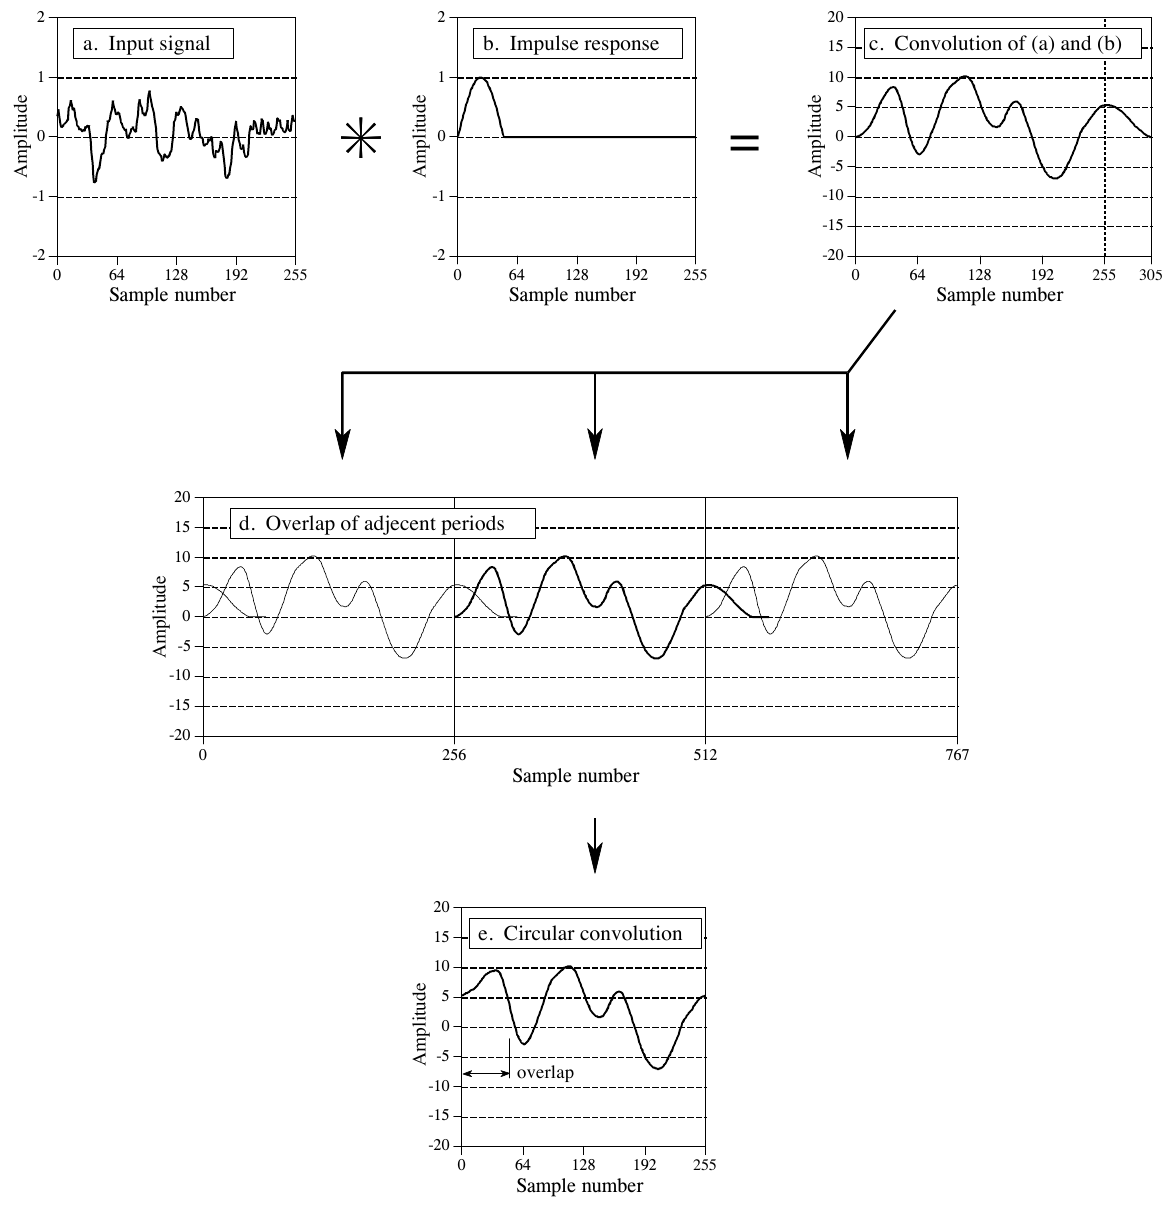
\includegraphics[width=0.971\linewidth,height=0.8\textheight,keepaspectratio]{assets/ch09/fig9-09.png}
\caption*{\textbf{图 9-9　循环卷积。} 256 个采样的信号 (a) 与 51 个采样的冲激响应
(b) 卷积，得到 306 个采样的信号 (c)。如果用 256 点 DFT
在频域中做这个卷积，正确卷积结果的 306 个点放不进提供的 256 个采样里。如
(d) 所示，输出信号的第 256 到 305
个采样被推进右边的下一个周期，与下一周期信号的开头相加。(e)
是所得信号的一个周期。 （a. Input signal = 输入信号；b. Impulse response
= 冲激响应；c.~Convolution of (a) and (b) = (a) 与 (b)
的卷积；d.~Overlap of adjecent periods = 相邻周期的重叠（adjecent
为原书拼写错误，应为 adjacent）；e. Circular convolution =
循环卷积；overlap = 重叠部分。Amplitude = 幅度，Sample number =
采样序号。）}
\end{figure}

要理解循环卷积，记住 N 点 DFT 把时域看作一个无限长的周期信号，每个周期 N
个采样。图 (d) 画出了本例中 DFT 眼里输出信号的三个周期。由于 N =
256，每个周期有 256 个点：0～255、256～511 和 512～767。频域卷积试图把
(c) 中 306 点的正确输出信号放进每个 256 点的周期里。结果有 49
个采样被推进右边相邻的周期，与本来就在那里的采样重叠。这些重叠部分相加，使每个周期都呈现为
(e) 的样子，也就是循环卷积。

\begin{quote}
\textbf{译注：} 按图注，被推出去的是第 256 到 305 个采样，共 306 − 256 =
50 个，正文写的 49 个应为 50 个。
\end{quote}

一旦理解了循环卷积的本质，避开它就很容易了。只要给参与卷积的每个信号补足够多的零，让输出信号有空间容纳正确卷积结果的
N + M − 1 个点。例如，可以把 (a) 和 (b) 中的信号补零到 512 点长，然后用
512 点 DFT。做完频域卷积后，输出信号由 306 个非零采样加上 206
个值为零的采样组成。第 18 章会详细讲解这个过程。

为什么叫循环卷积？回头看图 9-9d，考察中间那个周期，即第 256 到 511
个采样。由于所有周期都一样，从这个周期右边流出去的那部分信号，和从左边流进这个周期的那部分是一样的。如果只考虑单个周期，比如
(e)，看起来信号的右边不知怎么和左边连在了一起。想象一条咬住自己尾巴的蛇：第
255 个采样紧挨着第 0 个采样，就像第 100 个采样紧挨着第 101
个采样一样。信号的一部分从右边出去时，会神奇地从左边重新出现。换句话说，N
点时域的行为就像它是一个圆环。

上一章我们提出过一个问题：把 DFT 的时域看作 N 个点，还是看作周期为 N
的无限长周期信号，真的有区别吗？循环卷积就是一个有区别的例子。如果把时域信号理解为周期性的，循环卷积中遇到的失真就可以简单地解释为信号从一个周期扩展到了下一个周期。相比之下，如果只考虑时域的
N
个点，就会得出一个相当离奇的结论：频域卷积的作用就好像时域不知怎么卷成了一个圆环，第
0 个采样紧挨着第 N−1 个采样。
